\subsection{Calculating the total enhancement}

To get the total enhancement in the square simulated area equation \ref{eq:enhancement} can be used. The measured enhancement of this area will be the mean of the values within the slice.

\begin{figure}[!h]
  \centering
  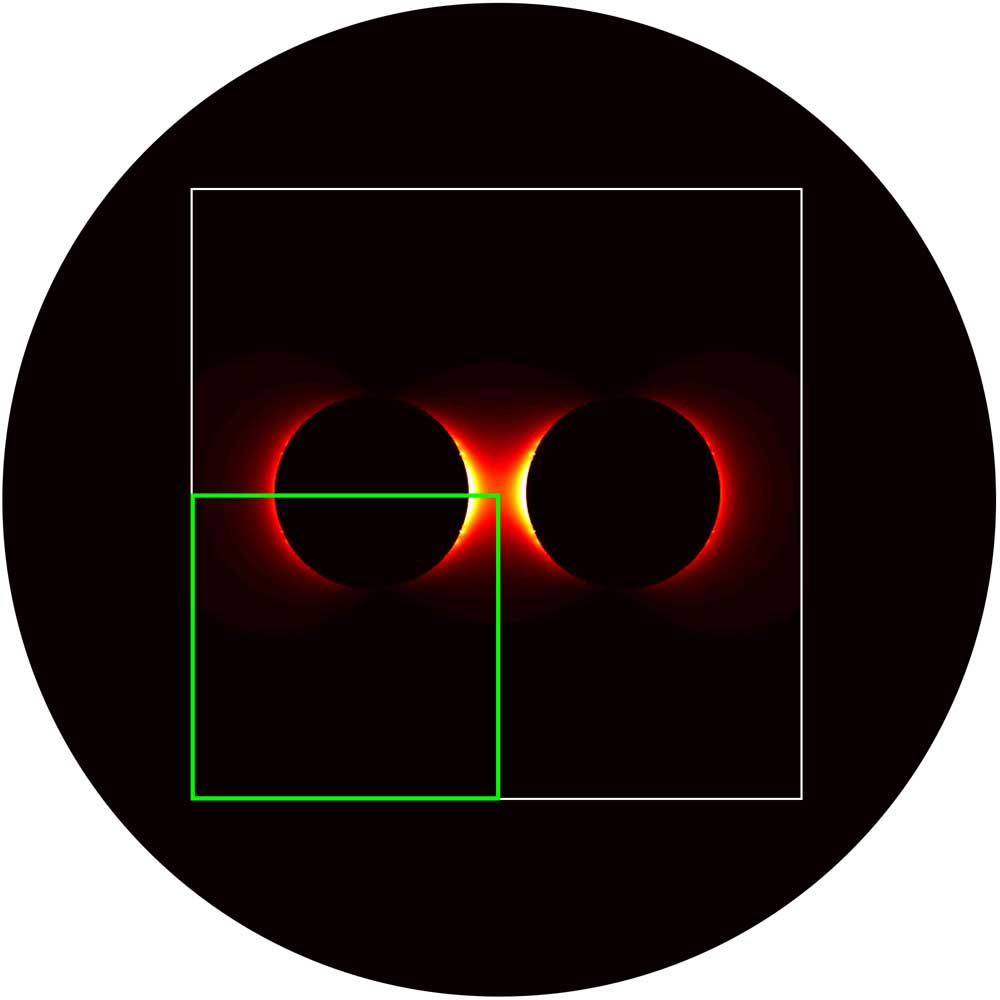
\includegraphics[width=0.5\textwidth]{./images/fwhm-chart.jpg}
  \label{fig:symmetry}
  \caption{The simulated square area (green box) compared to the calculated area (white box) compared to the total area measured by the laser (approximated as circle). The laser has a fwhm of \SI{570}{nm} according to \cite{heeg}.}
\end{figure}

This average value leads to $60.2$ for the \SI{2}{nm} corner size, $60.2$ for the \SI{5}{nm} corner size (both in the plane of graphene) and $59.2$ for the \SI{5}{nm} corner size for a planar slize at $z=\SI{40}{nm}$. The similarity between these values already shows that the estimation of \cite{heeg} to use the $z=\SI{40}{nm}$ plane is pretty good.

There is one last factor be taken into account: The used laser with a fwhm of \SI{570}{nm} can be estimated with a circle of radius \SI{285}{nm}. This circle has an area of \SI{255 180}{nm^2} which leads compared with the simulated area of \SI{160 000}{nm^2} to $62.7\%$ contribution of the simulated area to the total enhancement as seen in figure \ref{fig:symmetry}.

The area around the simulated area is approximated as the mean of the outer points of the simulated area.

Taking the laser geometry into account the resulting enhancements are $38.1$ for the \SI{2}{nm} corner size, $37.8$ for the \SI{5}{nm} corner size (both in the plane of graphene) and $37.2$ for the \SI{5}{nm} corner size for a planar slize at $z=\SI{40}{nm}$

\subsection{Spatial coherence in near-field Raman scattering}

While classically Raman scattering is treated as a spatially incoherent process which means that spatially distinct locations are considered as uncorrelated and the scattered signal is proportional to the scatterers volume. A recent publication has proven that at nanoscale this assumption does not hold and there is a correlation length of about \SI{30}{nm} for Raman scattering in graphene \cite{coherence}.

To account for this effect the outgoing enhancement has to be adapted. The easiest approximation is to take the mean of a radius of \SI{30}{nm} around each point instead of the point's value directly, effectively blurring the slice as shown in figure~\ref{fig:coherence}.

\begin{figure}[!h]
  \centering
  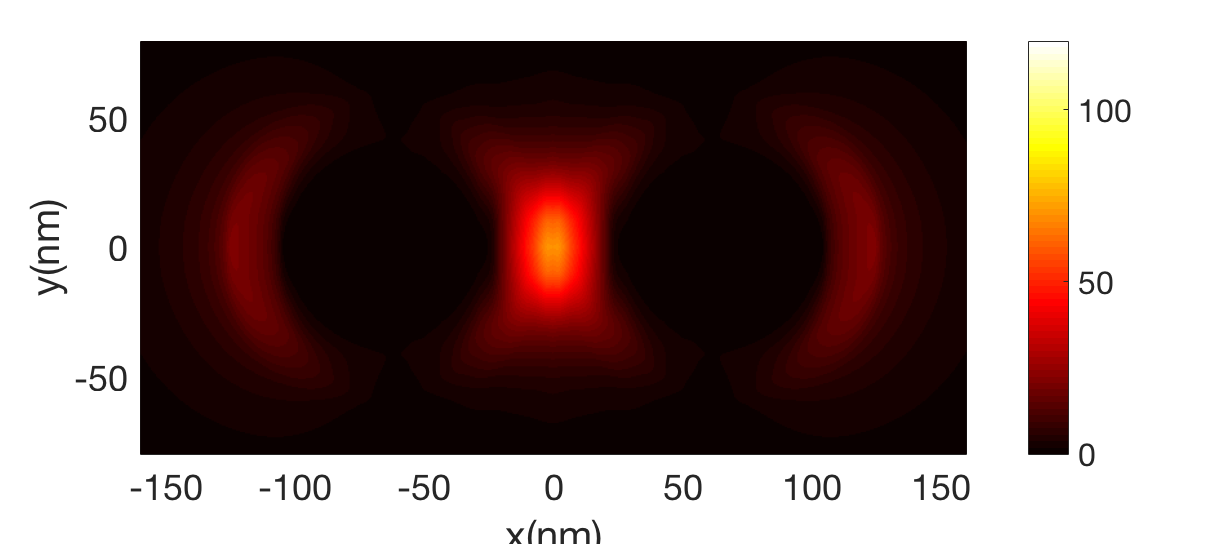
\includegraphics[width=0.8\textwidth]{./images/coherence.png}
  \caption{Outgoing local enhancement for a $z=\SI{40}{nm}$ slice. Due to the spatial coherence effect in near-field Raman scattering the outgoing enhancement is effectivly blurred with a radius of \SI{30}{nm} which decreases the total enhancement.}
  \label{fig:coherence}
\end{figure}

Taking this approximation into account for the \SI{40}{nm} slice the total enhancement decreases to $23.0$.
